\section{Implementation}
This section will describe the process of implementing BX between a RE and a DFA. It will start by describing the reasoning about how to implement the BX and will follow by explaining the implementation process, including the explanation about the algorithm's choices. Finally, it will present the \textit{put} strategy defined for a BX between NDFA and DFA.

The source code of the implementation is available in the Github repository:  \url{https://github.com/lisandrasilva/rv-bx}.

\subsection{Reasoning about BX}
Considering the already existent algorithms to convert between a RE and a DFA, we decided to attempt implementing the BX as a composition of two small BX, more concretely, one between RE and NDFA and another between NDFA and DFA. As depicted in Figure \ref{fig:BX} the NDFA would be an intermediate structure used as a view in one of the BX and as a source in the another.  

\begin{figure}
    \centering
    \resizebox{.4\textwidth}{!}{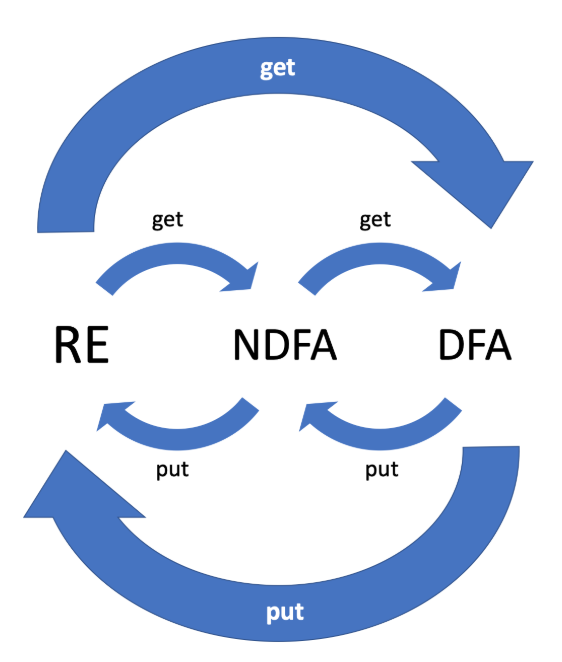
\includegraphics{Images/BX_arc.png}}
    \caption{BX between RE and DFA}
    \label{fig:BX}
\end{figure}

In the BX between RE and NDFA the source is the RE and the view is the NDFA. The \textit{getNDFA} function from RE to NDFA would be one of the conversion algorithms presented on Section \ref{convert} - Thompson's construction or Glushkov's construction. Regarding the BX between NDFA and the DFA, the source is the NDFA and the view is the DFA, where the \textit{getDFA} function would be the Powerset construction algorithm.

\vspace{5mm}
The \textit{get} function that given a RE as source and produces a DFA as view will be the composition of these two functions:

\begin{center}
    \textit{\textbf{get re} = (getDFA . getNDFA) re}
\end{center}

\vspace{5mm}
The main goal is to define the \textit{putback} functions:

\vspace{3mm}
\textbf{\textit{putNDFA}} - function that accepts a NDFA as a source and a possible modified DFA as a view and reflects the changes on the view into the source;
    
\textbf{\textit{putRE}} - function that accepts a RE as a source and a possible modified NDFA as a view and reflects the changes on the view into the source.

\vspace{5mm}
The final \textit{putback} function that accepts a RE as a source and a possible modified DFA as a view and produces the updated RE will be the composition of these two functions:


\begin{center}
    \textit{\textbf{put re dfa} = putRE re (putNDFA (get re) dfa)}
\end{center}

To tackle the problem we decided to start by define the \textit{putNDFA} function.

\subsection{Get function}
As said above the \textit{get} function will be the composition of two, with a NDFA as an intermediate structure. Once this NDFA will be the source argument of the \textit{putNDFA} function and the view argument for the \textit{putRE} function, it is necessary to reason about what type of NDFA we should consider, which means reason about the choice for the \textit{getNDFA} function.

The NDFA can be obtained through the Thompson's construction algorithm or through the Glushkov's construction algorithm. But, recall that the resulting NDFA are different since the one obtained through Glushkov's algorithm is \textit{$\epsilon$-free}, while the one obtained through the Thompson's algorithm has $\epsilon$-transitions. 

\subsubsection{NDFA with $\epsilon$-transitions}
Let's consider the NDFA in Figure \ref{fig:epsilon} and its correspondent DFA in Figure \ref{fig:epsilondfa} obtained through the Powerset construction algorithm. 

\begin{figure}
    \centering
    \resizebox{.7\textwidth}{!}{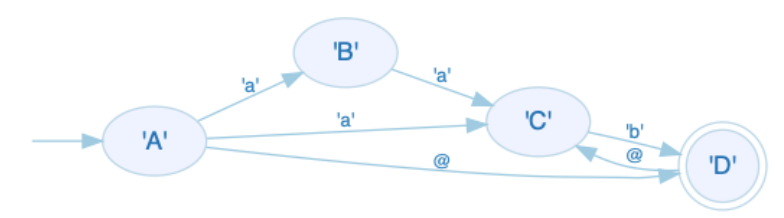
\includegraphics{Images/epsilondfa.png}}
    \caption{NDFA with $\epsilon$-transitions}
    \label{fig:epsilon}
\end{figure}

\begin{figure}
    \centering
    \resizebox{.7\textwidth}{!}{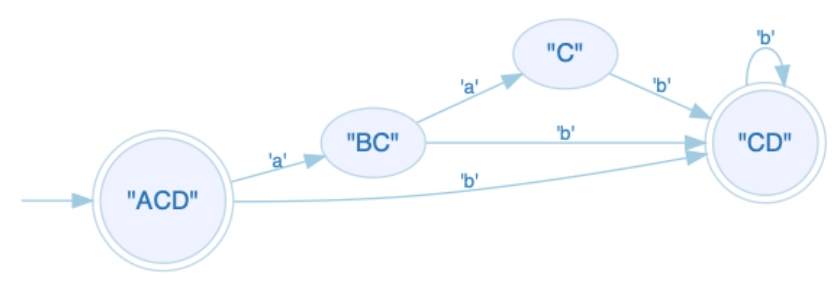
\includegraphics{Images/epsilon_DFA.png}}
    \caption{DFA obtained from NDFA in Figure \ref{fig:epsilon}}
    \label{fig:epsilondfa}
\end{figure}

By analyzing  the pictures is very hard to reason about a \textit{putback} function when the NDFA has $\epsilon$-transitions. For instance, in the obtained DFA of the given example (Figure \ref{fig:epsilondfa}) all the nodes are dependent on the transitions of the 'C' node in the NDFA, which means that when adding or removing transitions from or to node 'C' in the NDFA, this changes will be reflected in all the nodes with 'C' in the DFA (because that is what is demanded by the Powerset construction).

This fact restricts too much the possible changes in the view, and even though we designed a pseudo-algorithm to \textit{put} function in many cases it didn't satisfied the GetPut law. 

\subsubsection{NDFA \textit{$\epsilon$-free}} Figure \ref{fig:glundfa} depicts a NDFA \textit{$\epsilon$-free} equivalent to the NDFA in Figure \ref{fig:epsilondfa} and in Figure \ref{fig:gludfa} its the correspondent DFA. 

\begin{figure}[H]
    \centering
    \resizebox{.8\textwidth}{!}{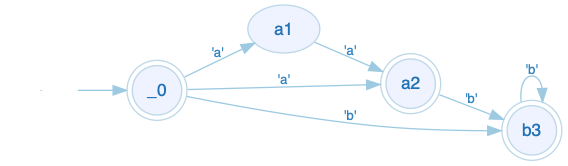
\includegraphics{Images/Glushkovdot.png}}
    \caption{NDFA \textit{$\epsilon$-free}}
    \label{fig:glundfa}
\end{figure}

\begin{figure}
    \centering
    \resizebox{.8\textwidth}{!}{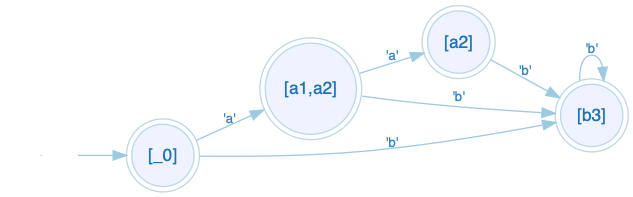
\includegraphics{Images/gluDFAdot.png}}
    \caption{DFA obtained from NDFA in Figure \ref{fig:epsilon}}
    \label{fig:gludfa}
\end{figure}

As we can conclude by analyzing the two automata, there are less dependencies, the only dependency is between nodes \texttt{[a1,a2]} and \texttt{[a2]}, because both have the node \texttt{a2} from the NDFA, therefore changes in this node will be reflected in both nodes in the view, even only one was modified in the first place. 

However, as it allows a wider range of possible changes on the view we decided to choose the \textit{$\epsilon$-free} NDFA to define the \textit{put} strategy between NDFA and DFA, which means that the \textit{get} function from RE to NDFA should be the Glushkov's construction algorithm. 

\subsection{Put back from DFA to NDFA}

\subsubsection{Structures for DFA and NDFA}
When reasoning about the put back function, the first step was to define the structures to represent both the NDFA and the DFA. Both structures are structurally very similar, but they will differ in the transition table \texttt{delta}, since in the DFA is not allowed to have two transitions from the same node with the same symbol, while in the NDFA that is possible. 

\begin{verbatim}
data Ndfa st sy = Ndfa { vocabularyN :: [sy ],
                         statesN     :: [st ],
                         initialSN   :: [st ],
                         finalSN     :: [st ],
                         deltaN      :: [((st,sy),st)]
                       }
                   
data Dfa st sy = Dfa { vocabularyD :: [sy],
                       statesD     :: [st],
                       initialSD   :: st,
                       finalSD     :: [st],
                       deltaD      :: [((st,sy),st)]
                     }
\end{verbatim}

We decided to represent the structures with polymorphism on the arguments so they can be more flexible on the types they can represent. However, remind that in the present work, the DFA is result of the Powerset construction of the NDFA, which means that the states in the DFA are sets of the states in the NDFA. As so, if in NDFA the type of \texttt{st} is for example \texttt{Int}, then the type of \texttt{st} in the DFA is \texttt{[Int]}. 

Table \ref{tablestruct} shows how the automata in Figures \ref{fig:glundfa} and \ref{fig:gludfa} are (pretty-printed) represented in the data structures mentioned above.

\begin{table}
  \begin{center}
    \begin{tabular}{ | p{3cm} |p{4cm}||p{4cm}|  }
    \hline
         & NDFA & DFA \\ [1ex]
        \hline
        \hline
        Vocabulary & `b', `a' & `b', `a'\\ [0.7ex]
        \hline
        States & \_0, b3, a2, a1 & [a2], [a1,a2], [b3], [\_0]\\ [0.7ex]
        \hline
        Initial State & \_0 & [\_0] \\ [0.7ex]
        \hline
        Final States & \_0, a2, b3 & [a2], [a1,a2], [b3], [\_0] \\ [0.7ex]
        \hline
        \multirow{3}{5em}{Transition Table} & \_0 $\xrightarrow{'a'}$ a1 & [\_0] $\xrightarrow{'a'}$ [a1,a2]\\
        & \_0 $\xrightarrow{'b'}$ a2 & [\_0]    $\xrightarrow{'b'}$ [b3]\\
        & \_0 $\xrightarrow{'b'}$ b3 & [a1,a2]  $\xrightarrow{'a'}$ [a2]\\
        & a1  $\xrightarrow{'b'}$ a2 & [a1,a2]  $\xrightarrow{'b'}$ [b3]\\
        & a2  $\xrightarrow{'b'}$ b3 & [a2]     $\xrightarrow{'b'}$ [b3]\\
        & b3  $\xrightarrow{'b'}$ b3 & [b3]     $\xrightarrow{'b'}$ [b3]\\
        \hline
        \end{tabular}
  \end{center}
  \caption{Representation of automata in Figures \ref{fig:glundfa} and \ref{fig:gludfa}}
  \label{tablestruct}
\end{table}

\subsubsection{Reflecting transition table}
The function \texttt{getTable} is responsible for reflecting the DFA transition table into the NDFA transition table. Therefore, it receives as argument the NDFA transition table, the DFA transition table and the set of states $q$ of the DFA (to perform checks) and returns the updated NDFA transition table. The argument with the DFA transition table is in fact zipped with an accumulator that will save, for each DFA transition $os \xrightarrow{s} ds$, the subset of $ds$ of the NDFA transitions that were validated so far. Following is the code but this will be better understood with the example given afterwards. 

\begin{verbatim}
getTable :: (Ord st, Ord sy) =>[((st,sy),st)] 
                             ->[((([st],sy),[st]),[st)]
                             -> [[st]] 
                             ->[((st,sy),st)]
getTable [] dfaT q = 
    let toAdd = filter (not . null . snd)
                [(((os,d),ds\\rs)) |(((os,d),ds),rs) <- dfaT]
    in concat $ map (`rearrangeS' q)toAdd
    
getTable (t@((o,s),d):ts) dfaT q = 
    let relS = [ x | x <- q , o `elem' x]
        trns = [ 1 | (((os,sym),ds),rs) <- dfaT , 
                                           os `elem' relS ,
                                           sym == s , 
                                           d `elem' ds]
        dfaT' = map (updateListAux t) dfaT
    in if (length relS == length trns) && (not $ null relS) 
       then t:getTable ts dfaT' q
       else getTable ts dfaT q
\end{verbatim}

\vspace{5mm}
%The function consumes each NDFA transition table recursively. 
For each NDFA transition \texttt{((o,s),d)}, the function verifies that each node in the DFA that contains `$o$' has the transition through symbol `$s$' for a node that contains `$d$'. When this is valid then the NDFA transition is kept in the source and the `$d$' is added to the auxiliary list from the DFA transitions mentioned above (using \texttt{updateListAux} function), otherwise is discarded. 



\begin{verbatim}
updateListAux ((o,s1),d)(((os,s2),ds),rs) = 
            if o `elem' os && s1 == s2 &&d `elem' ds
            then (((os,s2),ds),d:rs)
            else (((os,s2),ds),rs)
\end{verbatim}

Going back to the example in Figures \ref{fig:glundfa} and \ref{fig:gludfa}, let's do the following sequence of modifications on the view (depicted in DFA in Figure \ref{fig:updatedfa}):

\begin{itemize}
    \item Remove transition [a2] $\xrightarrow{'b'}$ [b3]
    \item Add transition [a1,a2] $\xrightarrow{'c'}$ [c4]
    \item Add transition [c4] $\xrightarrow{'b'}$ [b3]
\end{itemize}


\begin{figure}
    \centering
    \resizebox{.85\textwidth}{!}{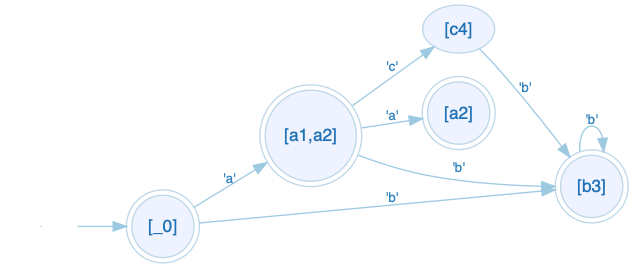
\includegraphics{Images/updatedDFA.png}}
    \caption{Updated view}
    \label{fig:updatedfa}
\end{figure}

Table \ref{getTable} represents the arguments to the function \texttt{getTable} with the updated DFA transition table.
As mentioned, the function \texttt{getTable} goes recursively through the NDFA transitions. For the first NDFA transition \texttt{((\_0,'a'),a1)} the function gets all the DFA states that contain \_0, which is only [\_0], and ensures that it has the transition through 'a' to a node which contains a1. As this is true due to transition \texttt{(([\_0],'a'),[a1,a2])} then a1 is added to the auxiliary accumulator list of the transition.

\begin{table}[H]
  \begin{center}
    \begin{tabular}{ | p{3cm} |p{4cm}||p{3cm} p{1cm} |  }
    \hline
         & NDFA & DFA & \\ [1ex]
        \hline
        States & \_0, b3, a2, a1 & [a2], [a1,a2], [b3], [\_0], & [c4] \\ [0.7ex]
        \hline
        \multirow{3}{5em}{Transition Table} & \_0 $\xrightarrow{'a'}$ a1 & [\_0] $\xrightarrow{'a'}$ [a1,a2] & [ ]\\
        & \_0 $\xrightarrow{'b'}$ a2 & [\_0]    $\xrightarrow{'b'}$ [b3] & [ ]\\
        & \_0 $\xrightarrow{'b'}$ b3 & [a1,a2]  $\xrightarrow{'a'}$ [a2] & [ ]\\
        & a1  $\xrightarrow{'b'}$ a2 & [a1,a2]  $\xrightarrow{'b'}$ [b3] & [ ]\\
        & a2  $\xrightarrow{'b'}$ b3 & \textcolor{gray}{[a2]     $\xrightarrow{'b'}$ [b3]} &  \\
        & b3  $\xrightarrow{'b'}$ b3 & [b3]     $\xrightarrow{'b'}$ [b3] & [ ]\\
        &  & \textcolor{ForestGreen}{[a1,a2]  $\xrightarrow{'c'}$ [c4]} & \textcolor{ForestGreen}{[ ]}\\
        &  & \textcolor{ForestGreen}{[c4]  $\xrightarrow{'b'}$ [b3]} & \textcolor{ForestGreen}{[ ]}\\
        \hline
        \end{tabular}
  \end{center}
  \caption{Arguments for \texttt{getTable} with updated view}
  \label{getTable}
\end{table}

When analyzing NDFA transition \texttt{((a2,'b'),b3)}, all the DFA nodes that contain \texttt{a2} (\texttt{[a1,a2]} and \texttt{[a2]}) must have the transition through \texttt{'b'} to a node that contains \texttt{b3}. However this is not verified since the DFA transition \texttt{(([a2],'b'),[b3])} was removed from the view, therefore this NDFA transition is not kept in the source.


\begin{table}[H]
  \begin{center}
    \begin{tabular}{ | p{3cm} |p{4cm}||p{3cm} p{1cm} |  }
    \hline
         & NDFA & DFA & \\ [1ex]
        \hline
        States & \_0, b3, a2, a1 & [a2], [a1,a2], [b3], [\_0], & [c4]\\ [0.7ex]
        \hline
        \multirow{3}{5em}{Transition Table} & \textcolor{blue}{\_0 $\xrightarrow{'a'}$ a1} & [\_0] $\xrightarrow{'a'}$ [a1,a2] & [\textcolor{blue}{a1,a2}]\\
        & \textcolor{blue}{\_0 $\xrightarrow{'b'}$ a2} & [\_0]   $\xrightarrow{'b'}$ [b3] & [\textcolor{blue}{b3}]\\
        & \textcolor{blue}{\_0 $\xrightarrow{'b'}$ b3} & [a1,a2]  $\xrightarrow{'a'}$ [a2] & [\textcolor{blue}{a2}]\\
        & \textcolor{blue}{a1  $\xrightarrow{'b'}$ a2} & [a1,a2]  $\xrightarrow{'b'}$ [b3] & [ ]\\
        & \textcolor{gray}{a2  $\xrightarrow{'b'}$ b3} & \textcolor{gray}{[a2]     $\xrightarrow{'b'}$ [b3]} &  \\
        & \textcolor{blue}{b3  $\xrightarrow{'b'}$ b3} & [b3]     $\xrightarrow{'b'}$ [b3] & [\textcolor{blue}{b3}]\\
        &  & \textcolor{ForestGreen}{[a1,a2]  $\xrightarrow{'c'}$ [c4]} & \textcolor{ForestGreen}{[ ]}\\
        &  & \textcolor{ForestGreen}{[c4]  $\xrightarrow{'b'}$ [b3]} & \textcolor{ForestGreen}{[ ]}\\
        \hline
        \end{tabular}
  \end{center}
  \caption{Transition tables after \texttt{getTable} processed all old NDFA transitions}
  \label{getTable2}
\end{table}

Table \ref{getTable2} contains the state of the transition tables after the function \texttt{getTable} already processed all the NDFA transitions. After that, the function \texttt{getTable} is recursively called with the first argument (NDFA table transtion) empty. At this point, for each DFA transition \texttt{((os,s),ds)} its corresponding auxiliary list with the subset of $ds$ that were already validated is removed from the set $ds$. If the remaining $ds$ list is empty then it means that the transition was already validated. When there are still states in the $ds$ list the new transitions in the NDFA must be created (Table \ref{getTable3}). This is done in the \texttt{rearrangeS} function. 

\begin{table}
  \begin{center}
    \begin{tabular}{ | p{3cm} |p{4cm}||p{3cm} p{1cm} |  }
    \hline
         & NDFA & DFA & \\ [1ex]
        \hline
        States & \_0, b3, a2, a1 & [a2], [a1,a2], [b3], [\_0], & [c4]\\ [0.7ex]
        \hline
        \multirow{3}{5em}{Transition Table} & \textcolor{blue}{\_0 $\xrightarrow{'a'}$ a1} & [a1,a2]  $\xrightarrow{'b'}$ [b3] & [ ]\\
        & \textcolor{blue}{\_0 $\xrightarrow{'b'}$ a2} & \textcolor{ForestGreen}{[a1,a2]  $\xrightarrow{'c'}$ [c4]} & \textcolor{ForestGreen}{[ ]}\\
        & \textcolor{blue}{\_0 $\xrightarrow{'b'}$ b3} & \textcolor{ForestGreen}{[c4]  $\xrightarrow{'b'}$ [b3]} & \textcolor{ForestGreen}{[ ]}\\
        & \textcolor{blue}{a1  $\xrightarrow{'b'}$ a2} & & \\
        & \textcolor{blue}{b3  $\xrightarrow{'b'}$ b3} & & \\
        \hline
        \end{tabular}
  \end{center}
  \caption{Transition tables before call \texttt{rearrangeS} function}
  \label{getTable3}
\end{table}

The function receives a DFA transition, the set of DFA states and creates the list of new NDFA transitions corresponding to the given DFA transition. 
First the function computes the minimum list of NDFA transitions, excluding transitions which origin appear in other DFA nodes. 

\begin{verbatim}
rearrangeS :: Eq st => (([st], sy), [st])
                    -> [[st]] 
                    -> [((st, sy), st)]
rearrangeS ((os,sy),dsts) q = 
    let min = [((o,sy),dd) | o <- os \\ (concat $ delete os q), 
                             dd <- dsts]
    in if null min then [((o,sy),dd) | o <- os, dd <- dsts]
       else min 
\end{verbatim}

For instance, when creating the new NDFA transitions for the DFA transition \texttt{(([a1,a2],'b'),[b3])} it is only desirable create the new transition \texttt{((a1,'b'),b3)} since if a transition from \texttt{a2} is also created then when \textit{getting} again the DFA, the node \texttt{[a2]} will also have the transition, that was not created by the user, leading to violation of the GetPut law. 

Sometimes it is not possible to create new transitions without violating the law, for instance if instead of the DFA transition \texttt{(([a1,a2],'b'),[b3])} we had \texttt{(([a2],'b'),[b3])}, the minimum computed list of the new NDFA transitions would be empty. This means that the edited view is not consistent with the source, because it is not possible to reflect the modifications without modify other node transitions. In this cases, the function returns all the possible transitions and the inconsistency will be handled later. 
%Table \ref{getablefinal} shows the updated NDFA transition table returned by the function \texttt{getTable}.

\begin{table}
  \begin{center}
    \begin{tabular}{ | p{3cm} | p{4cm}|  }
    \hline
         & NDFA \\ [1ex]
        \hline
        \hline
        \multirow{3}{5em}{Transition Table} & \_0 $\xrightarrow{'a'}$ a1\\
        & \_0 $\xrightarrow{'b'}$ a2 \\
        & \_0 $\xrightarrow{'b'}$ b3 \\
        & a1  $\xrightarrow{'b'}$ a2 \\
        & b3  $\xrightarrow{'b'}$ b3 \\
        & \textcolor{ForestGreen}{a1  $\xrightarrow{'b'}$ b3} \\
        & \textcolor{ForestGreen}{a1  $\xrightarrow{'c'}$ c4} \\
        & \textcolor{ForestGreen}{c4  $\xrightarrow{'b'}$ b3} \\
        \hline
        \end{tabular}
  \end{center}
  \caption{Updated NDFA transition table}
  \label{getablefinal}
\end{table}

%For instance, taking the last example, if a new DFA transition is added (([a1,a2],c),[c1]) only the NDFA transition ((a1,c),c1) must be created since if the transition ((a2,c),c1) is also created then when \textit{getting} again the view the DFA would also have the edge (([a2],c),[c1]), that was not created by the user, and so the GetPut law would not be satisfied. When the computed \texttt{min} list is empty it means that is not possible to create new edges without interfere with other DFA nodes, that is called an inconsistency with the source. In this case the function returns all possible NDFA edges for the respective DFA transition, and the inconsistency is dealed with later. 

\subsubsection{Updating NDFA Structure}
After the table transition of the NDFA is complete it is still necessary to update the other fields of the NDFA structure, this is done by the function \texttt{putNdfaStruct}.

The \textit{put} of the other fields of the structure is very straight, the most complex is the final states. For that, for each old final state the function tests if it still belongs to some of the new final states and in that case it is kept as a final state or discarded otherwise. In the end the remaining final states are added as final state. 

\begin{verbatim}
putNdfaStruct :: (Ord st, Ord sy) => Ndfa st sy  
                                  -> Dfa [st] sy 
                                  -> Ndfa st sy
putNdfaStruct (Ndfa v1 q1 s1 z1 d1) (Dfa v2 q2 s2 z2 d2) = 
        Ndfa v q s z d
    where v = v2
          q = nub $ concat q2
          s = s1
          z = f z1 (concat z2)
          d = getTable d1 (zip d2 (repeat [])) q2
          f [] cz2 = cz2
          f (h:t) cz2 = if h `elem` cz2 
                        then h:(f t (filter (/= h) cz2))
                        else f t cz2
\end{verbatim}

\vspace{5mm}
Table \ref{sourceUpdated} shows the updated NDFA (source) given the modified DFA (view), which is the result of the function \texttt{putNdfaStruct}.

\begin{table}[H]
  \begin{center}
    \begin{tabular}{ | p{3cm} |p{4cm}||p{4cm}|  }
    \hline
         & NDFA & DFA \\ [1ex]
        \hline
        \hline
        Vocabulary & `b', `a', \textcolor{ForestGreen}{`c'} & `b', `a', \textcolor{ForestGreen}{`c'}\\ [0.7ex]
        \hline
        States & \_0, b3, a2, a1, \textcolor{ForestGreen}{c4} & [a2], [a1,a2], [b3], [\_0], \textcolor{ForestGreen}{[c4]}\\ [0.7ex]
        \hline
        Initial State & \_0 & [\_0] \\ [0.7ex]
        \hline
        Final States & \_0, a2, b3 & [a2], [a1,a2], [b3], [\_0] \\ [0.7ex]
        \hline
        \multirow{3}{5em}{Transition Table} & \textcolor{blue}{\_0 $\xrightarrow{'a'}$ a1} & [\_0] $\xrightarrow{'a'}$ [a1,a2]\\
        & \textcolor{blue}{\_0 $\xrightarrow{'b'}$ a2} & [\_0]    $\xrightarrow{'b'}$ [b3]\\
        & \textcolor{blue}{\_0 $\xrightarrow{'b'}$ b3} & [a1,a2]  $\xrightarrow{'a'}$ [a2]\\
        & \textcolor{blue}{a1  $\xrightarrow{'b'}$ a2} & [a1,a2]  $\xrightarrow{'b'}$ [b3]\\
        & \textcolor{blue}{b3  $\xrightarrow{'b'}$ b3} & [b3]     $\xrightarrow{'b'}$ [b3]\\
        & \textcolor{ForestGreen}{a1  $\xrightarrow{'b'}$ b3} & \textcolor{ForestGreen}{[a1,a2]  $\xrightarrow{'c'}$ [c4]}\\
        & \textcolor{ForestGreen}{a1  $\xrightarrow{'c'}$ c4} & \textcolor{ForestGreen}{[c4]  $\xrightarrow{'b'}$ [b3]}\\
        & \textcolor{ForestGreen}{c4  $\xrightarrow{'b'}$ b3} & \\
        \hline
        \end{tabular}
  \end{center}
  \caption{Representation of automata in Figures \ref{fig:glundfa} and \ref{fig:gludfa}}
  \label{sourceUpdated}
\end{table}

\subsubsection{Well built DFA}
As the DFA can be edited by the user, and this changes will be reflected in the NDFA, it is important to guarantee that the DFA is well built before proceed with the \textit{put} function. This is guaranteed by the function \texttt{wellBuilt} that ensures the following:

\begin{itemize}
    \item Every transition from a given origin $o$ with a symbol $s$ is unique;
    \item Every Node $x$ must be reachable from the start node;
    \item Every node must reach an accepting node;
    \item For every transition $o \xrightarrow{s} d $, each state in the destination's list of $d$ states must be prefixed by the symbol $s$ (considering the NDFA is result of Glushkov's algorithm and DFA is result of Powerset construction);
    \item The initial state cannot be modified (also a requirement of Glushkov's algorithm)
\end{itemize}

The function returns an error message for each one of the above mentioned rules in case they are violated. 

\subsubsection{Put NDFA}
Finally, the function \texttt{putNDFA} puts it all together: it receives the NDFA, the (possibly) updated DFA and returns an \texttt{Error NDFA}. The \texttt{Error NDFA} is a data type that can contain the (updated) NDFA if everything went well or an error message in case the given DFA was not a valid DFA. The verification of the validity of DFA is done by the function \texttt{wellBuilt} that returns an \texttt{Error Bool}, i.e. an \texttt{Ok True} case the DFA is valid or an \texttt{Error m} where \texttt{m} contains the error message.

\vspace{5mm}
\begin{verbatim}
putNdfa :: Ndfa (Indexed Char) Char 
        -> Dfa [Indexed Char] Char
        -> Error (Ndfa (Indexed Char) Char)
putNdfa ndfa dfa = case wellBuilt dfa of 
                    Ok True -> Ok (putNdfaStruct ndfa dfa)
                    Error m -> Error m
\end{verbatim}

Given this \texttt{put} algorithm if we call the function \texttt{putNdfa} with the NDFA and DFA represented in Table \ref{tablestruct} (unmodified view), the output will be the same NDFA (Figure \ref{fig:glundfa}), which means that the PutGet law is satisfied. 
If we call the function \texttt{putNdfa} with the NDFA and DFA represented in Table \ref{getTable} (updated view), and then call the \textit{get} function (powerset construction) the DFA produced will be the same (Figure \ref{fig:updatedfa}), which means that for the given example the GetPut law is satisfied. However, as mentioned before this doesn't happen when there is inconsistencies between source and view, next section explains how the program deals with them.  


\subsubsection{Inconsistencies}
Taking again the previous example, it was possible to remove the transition \texttt{(([a2],b),[b3])} without violating the GetPut law property. However if we had removed the transition \texttt{(([a1,a2],b),[b3])} this would result in an inconsistency, because if the transition \texttt{(([a2],b),[b3])} still exists, it means that the NDFA will have the transition \texttt{((a2,b),b3)} and by the Powerset construction algorithm the transition \texttt{(([a1,a2],b),[b3])} will still be there.

When an inconsistency occurs in the view, it means that is not possible to get the same view with the updated source, because the dependencies in the view were not `respected'. In this cases, the user is asked if he wants to proceed with the consistent version of the view, and in that case the source is updated with the consistent version of the view.


\subsubsection{Interpreter}
It was also created an interpreter to interact with the user. The interpreter allows the user to perform a sequence of modifications on the view, that are displayed in graphs so the user can see the updated being done.
The possible modifications that the user can perform are:

\begin{itemize}
    \item Add transition;
    \item Remove transition;
    \item Remove node;
\end{itemize}

At any point the user can call the the \textit{put}, even when he had not performed any modification. In case the sequence of modifications result in an updated view that is not consistent with the source, the interpreter asks the user if he wants to continue or to rollback, in case he wants to continue the source is updated with the consistent version of the view, otherwise the modifications are discarded.
